%!TEX root = ../main.tex
\chapter{État de l'art}

Comme vous l'aurez compris, deux sujets principaux seront abordés dans ce mémoire : la gestion de la sécurité informatique
dans une chaîne de production DevOps et la gestion opérationnelle de la sécurité de cluster Kubernetes. 

Il me semble donc pertinent de dresser un état de l'art pour ces deux sujets afin de permettre une meilleure compréhension des
de leurs problématiques, mais aussi afin à mieux appréhender les possibles solutions à ces dernières.

\section{Evaluation des risques de sécurité}
\subsection{Les risques du Pipeline DevOps}

Dans la méthodologie DevOps, le \emph{Pipeline} est un concept regroupant des notions théoriques et socle technique utilisés dans 
le cadre d'un développement logiciel. Ainsi, l'utilisation du terme \emph{Pipeline} fait ainsi reférence au \ac{SDLC}
\autocite[Ch.\ 6]{devops_for_dummies_freeman_forsgren_2019}, aux standards de développement
\autocite[Ch.\ 9]{devops_for_dummies_freeman_forsgren_2019}, processus de qualification et 
validation, de même qu'à l'ensemble des outils et services utilisés par les équipes de développement. Il s'agit donc d'un élément
centrale dans la chaîne de production DevOps: tout problème impactant un élément du \emph{Pipeline} aura des répercussions sur les 
autre et risque ainsi de mettre en péril les opérations de développement.

Nous pouvons donc nous poser la question de la nature de ces risques et particulièrement de ceux relatifs à la sécurité du 
\emph{Pipeline}. Pour cela, nous allons utiliser comme support le \ac{SDLC} d'un logiciel afin de mieux cibler les problématiques
de sécurité à chaque étape d'un projet.

\vspace{2em}
\begin{figure}[h]
    \centering
    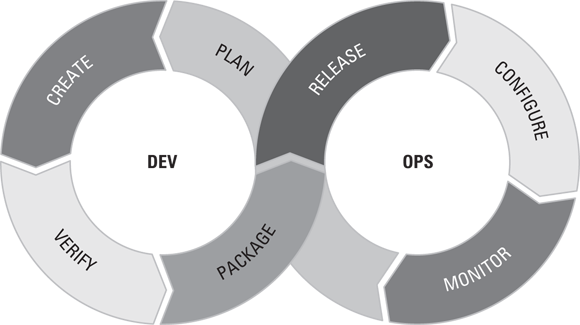
\includegraphics[width=0.5\linewidth]{resources/img/devops_lifecycle.png}
    \captionsource{Représentation du cycle de vie d'un projet DevOps}{DevOps for Dummies, Figure 6-1}
    \label{fig:devops-lifecycle}
\end{figure}
\newpage

Après une rapide analyse, voici les principaux risque qui se présente à nous :
\begin{multicols}{2}
    \begin{enumerate}
        \item Plan :
        \begin{itemize}
            \item Intégration d'une technologie vulnérable ou non maintenue
            \item Non-intégration de correctifs pour une vulnérabilité remontée
        \end{itemize}
        \item Create :
        \begin{itemize}
            \item Développement de code faïbles
            \item Mauvaise configuration du framework ou dépendances
        \end{itemize}
        \item Verify :
        \begin{itemize}
            \item Jeux de test incomplets
            \item Absence d'audit de sécurité applicative
        \end{itemize}
        \item Package :
        \begin{itemize}
            \item Utilisation d'un OS ou paquets vulnérables
            \columnbreak
            \item Erreur de configuration du conteneur
            \item Erreur de configuration des services
        \end{itemize}
        \item Release :
        \begin{itemize}
            \item Mauvaise gestion des versions de conteneurs
            \item Erreur de configuration du script de build
        \end{itemize}
        \item Configure :
        \begin{itemize}
            \item Mauvaise gestion des secrets
            \item Erreur de configuration des déploiements
        \end{itemize}
        \item Monitor :
        \begin{itemize}
            \item Absence ou trop faible collecte de log (application et conteneur)
        \end{itemize}
    \end{enumerate}
\end{multicols}

On constate donc que majoritairement les risques sont portés par des erreurs lors du développement.
Il s'agira donc d'un point d'attention dans la recherche de solutions.

\subsection{Les risques d'un cluster Kubernetes}

Bien que l'orchestrateur Kubernetes constitue une coûche d'abstraction entre l'infrastructure physique qui 
l'héberge et les conteneurs qu'il fait fonctionner, les risques qu'il porte sont similaires à une infrastructure
(virtualisé ou non) classique. Il est par exemple important de pouvoir lister les instances de conteneur (a.k.a. 
Pod) en cours d'execution, leur version ainsi que la présence de vulnérabilité; de pouvoir assurer un contrôle
d'accès approprié ou bien de pouvoir assurer la sécurité du réseau du cluster. 

Cependant, étant donné que le cluster se comporte comme une coûche d'abstraction, il hérite de problématiques
de sécurité qui lui sont propre. C'est ainsi qu'il est nécessaire de pouvoir surveiller les groupes de ressources
(Namespaces), de contraindre des configurations de déploiement ou l'origine des conteneurs.

\newpage

\section{Recherche de solutions}

Ayant maintenant identifiés les risques encourus par notre Pipeline DevOps et l'infrastructure Kubernetes associée,
nous pouvons nous intéresser aux solutions permettant leurs réduction.

Pour cela nous allons utiliser comme support la méthodologie décrite dans le \citetitle{samm_v2.0_owasp_project_2021}
\autocite{samm_v2.0_owasp_project_2021}
de l'\citeauthor{samm_v2.0_owasp_project_2021}. Cette méthodologie mis à jours en \citedate{samm_v2.0_owasp_project_2021}
fait office de référence pour l'analyse et l'amélioration de la sécurité des logiciels développés en entreprise; elle est
particulièrement recommandé dans le cadre de développement Agiles et / ou DevOps.

\subsection{Le modèle de référence}

Le \ac{SAMM} est, comme son nom l'indique, un modèle permettant de quantifier le niveau de maturité d'un processus de 
développement logiciel sur le plan de la sécurité informatique. Cette quantification est réalisée sur la base de différentes
pratiques de sécurité chacune regroupés dans des fonctions métier et notés sur une échelle de trois points avec en point 
initial zero implicite. Enfin, les pratiques de sécurité dispose de deux activité permettant de qualifier le niveau de 
maturité sur ses principaux thèmes.

Le \ac{SAMM} peu donc être représenté de la manière suivante :

\begin{figure}[h]
    \centering
    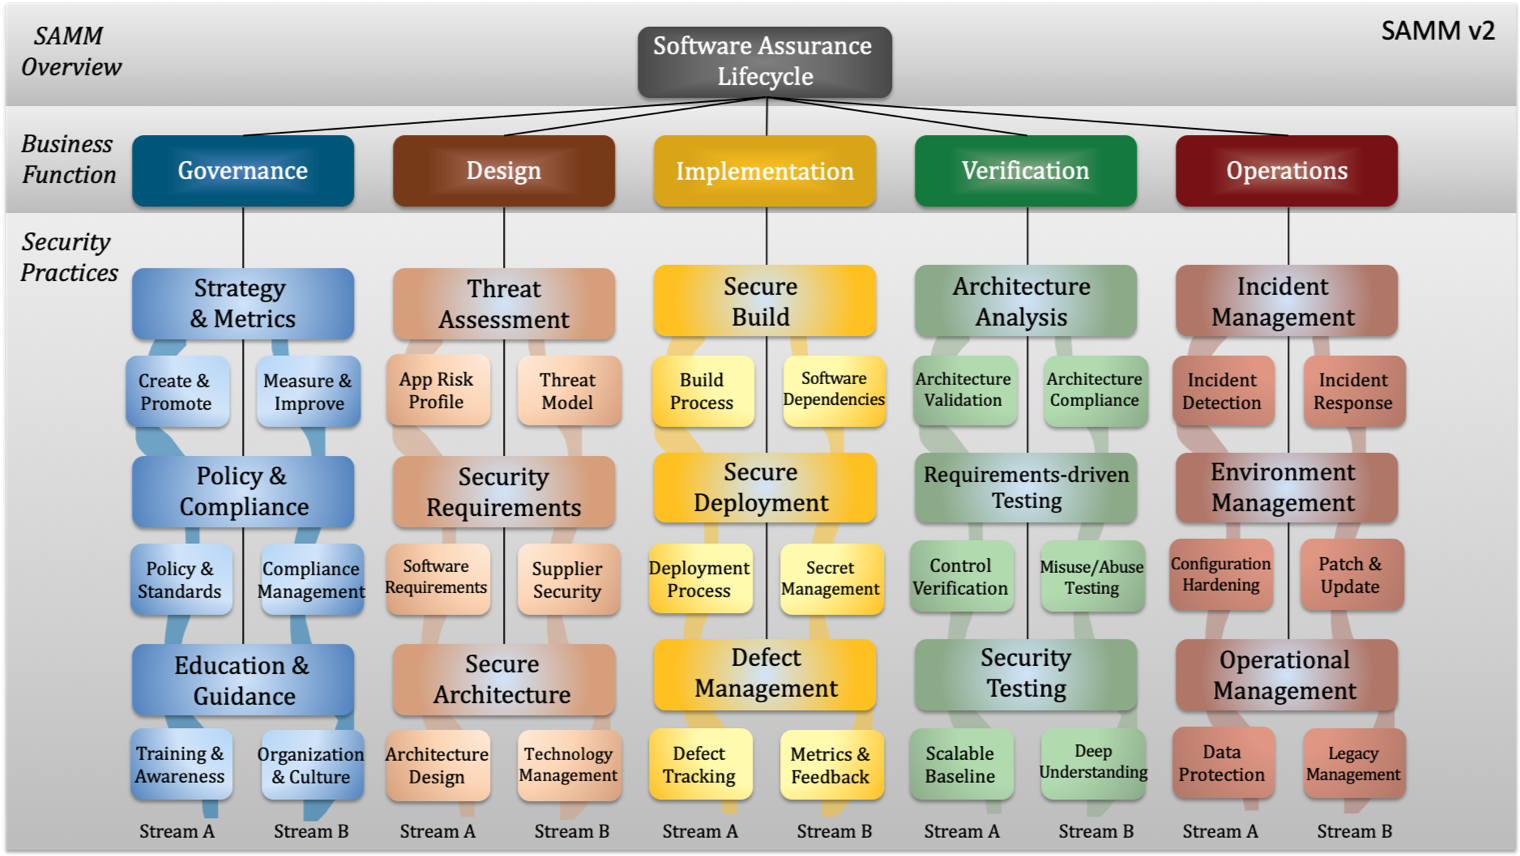
\includegraphics[width=1\linewidth]{resources/img/Samm_v2.png}
    \captionsource{Modèle SAMM v2}{Release note v2, \href{https://owaspsamm.org/release-notes-v2/}{OWASPSAMM.org}}
    \label{fig:samm-rep}
\end{figure}

\newpage

L'échelle de quantification quant à elle est défine de la manière suivante : 
\setlist[enumerate,1]{start=0}
\begin{enumerate}
    \item Niveau initial, aucune mesure de sécurité n'est appliqué.
    \item Niveau de compréhension basique de problématiques de sécurité et application de mesure ad hoc.
    \item Niveau avancé d'application des mesures de prévention avec constatation de l'efficacité ces dernières.
    \item Niveau de maîtrise complète des pratiques de sécurité à l'échelle de l'organisation.
\end{enumerate}
\setlist[enumerate,1]{start=1}
On considérera dans cette mission que le second niveau est un prérequis à la validation des pratiques de sécurité.
Le dernier niveau constitue quant à lui l'objectif à atteindre.

\subsection{Gouvernance}

La fonction \emph{Gouvernance}, telle que présentée dans le modèle \ac{SAMM}, représente le point de départ de la 
mise en oeuvre de la sécurité informatique dans le cadre de développement. C'est en effet grâce sur la base des 
trois pratiques de sécurité associés (\emph{Stratégie \& Métriques}, \emph{Politiquer \& Conformité}, 
\emph{Formation \& Conseils}) que seront issue l'ensemble des actions techniques et organisationnels des autres
fonctions métier.

La \emph{Gouvernance} de la sécurité des développement est un sujet déjà encrée dans la philosophie du Groupe JCDecaux.
Ainsi, il dispose d'un niveau de maturité avancé grâce notamment à la mise en place de politiques de sécurité dédiées
au développement et leur application, la formation et intégration d'interlocuteurs sensibilisé aux risques de sécurité
de même que la mise en place de \ac{KPI} permettant la mesure et l'amélioration de l'efficacité de la stratégie.
Cette stratégie, adoptant les principes de la sécurité par la conception (Security By Design) a par ailleurs fait 
l'objet d'une présentation\autocite{devopsrex_denis_2019} lors du \href{https://2019.devopsrex.fr/}{DevOpsREX 219} 
par Joy-Alexandra Denis, ex-RSSI du Groupe JCDecaux et maintenant RSSI de la filiale France du Groupe Ikea.

Cependant, et contrairement aux préconisations du \ac{NIST}\autocite*{app_cont_sec_nist_2017}, le Groupe ne dispose pas
d'une politique de sécurité dédié aux technologies de conteneurisation d'application et d'hébergement connexe. 

De même, bien que l'on observe une forte sensibilisation au problématiques de sécurité des responsable produit / projet, 
on constate que les populations de développeurs ne disposent pas d'un accompagnement spécifique institutionnalise au niveau
du groupe sur ces problématiques.
\newline Ainsi, le \ac{SAFECODE} recommande la formation continue des équipe de développement aux techniques de sécurisation
de code et au développement sécurisé dans son rapport \citetitle{six_pillarss_devsecops_safecode_2020} de 
\citedate{six_pillarss_devsecops_safecode_2020}.

\newpage

\subsection{Conception}

Si l'on considère que la \emph{Gouvernance} constitue les fondations d'un développement applicatif sécurisé, la conception et 
l'imagination de son architecture représente quant à lui l'ossature de cette dernière : une faiblesse dans la conception pourrait
entraîner la compromission globale de l'application. 
\newline Afin de prévenir ces risques, le modèle \ac{SAMM} propose trois axes de sécurisation : l'évaluation des risques, 
la définition de prérequis de sécurité et la sécurisation de l'architecture.

En 2019, l'équipe \ac{SSI} a réalisée une analyse de risque avec pour périmètre les développement réalisés pour le Groupe. 
Cette exercice, fortement inspiré par la méthodologie EBIOS Risk Manager \autocite{ebios_rm_anssi_2018}, a notamment favorisé 
la propagation du \emph{Security By Design} auprès des équipes de développement grâce à la présentation concrête des risques 
encourus par leurs applications et l'impacte qu'aurais un attaque sur celles-ci.

Cette même analyse de risque a permit de mettre à jours les prérequis de sécurité, tant logiciel qu'architecturaux, afin de les
ajuster aux nouvelles technologies exploités par le Groupe et ses filiales. Ainsi, les politiques d’\ac{IAM}
et de protection des données ont fait l’objet de mises à jours et intègrent maintenant les nouvelles réglementations Groupe 
vis-à-vis des services et technologies Cloud exploités.

\subsection{Implémentation}

La phase d'implémentation est l'une des phases les plus complexes dans un processus de développement. Il s'agit de l'étape
qui occupe la majorité du temps de développement d'une application car nécessitant la rédaction de centaines de lignes de 
code et tests associés.

Afin de veiller au bon déroulement de cette phase, ces mêmes développeurs mettent en oeuvre divers outils tel que du versionnage
de code, des tests automatiques et de la livraison automatique d'images\footnote{Ces outils de \ac{VCS}, \ac{CI}, \ac{CD} constituent
dans les fait la base technique du Pipeline DevOps.} que nous pouvons exploiter afin d'appliquer les trois pratiques de sécurité 
recommandé par la \ac{SAMM} : la détéction de défaut, la sécurisation des image et des déploiements.

Ainsi, il est possible d'étendre l'usage des outils de test automatique en ajoutant en intégrant de nouveaux jeux de test, dédiées à la 
détection d'erreurs d'implémentations.
C'est ce que propose par exemple les outils de \ac{DAST}  et \ac{IAST} tel que le service 
\href{https://www.rapid7.com/products/insightappsec/}{Rapid7 InsightAppSec} ou \href{https://www.acunetix.com/}{Acunetix d'Invicti}.

L'intégration de nouvelle règles orienté sécurité dans les outils d'analyse statique de code est elle aussi possible et permet d'intéger
des \ac{KPI} dans le contrôle qualité des développement.

Enfin, la sécurisation des image et de leur déploiement passe par l'automatisation des processus de build, l'analyse des dépendance et des
configuration pour finir par le blockage automatique de publication en cas de non conformité.

\subsection{Vérification}
